\documentclass[tikz,border=9pt]{standalone}
\usepackage{amsmath}
\usetikzlibrary{arrows.meta,calc,positioning}
\definecolor{walletblue}{HTML}{0072B2}
\definecolor{aggorange}{HTML}{D55E00}
\definecolor{verifygreen}{HTML}{009E73}
\begin{document}
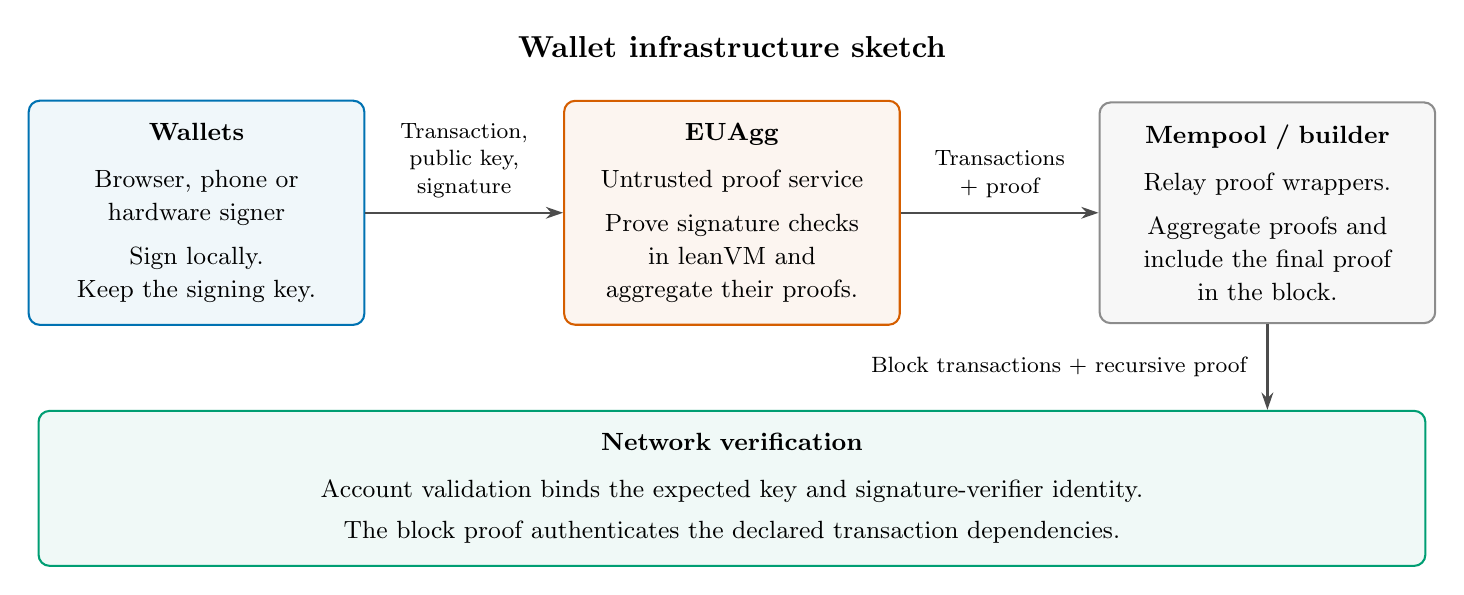
\begin{tikzpicture}[
  font=\fontsize{9.5}{12}\selectfont,
  box/.style={rounded corners=4pt,line width=.75pt,align=center,
    text width=3.7cm,minimum height=2.8cm,inner sep=8pt},
  arrow/.style={-{Stealth[length=2.2mm,width=1.5mm]},line width=.8pt,draw=black!70},
  label/.style={font=\fontsize{8}{10}\selectfont,align=center,fill=white,inner sep=2pt}
]
\node[font=\fontsize{11}{13}\selectfont\bfseries] at (6.8,2.1)
  {Wallet infrastructure sketch};

\node[box,draw=walletblue,fill=walletblue!6] (wallet) at (0,0)
  {\textbf{Wallets}\\[5pt]
  Browser, phone or\\hardware signer\\[4pt]
  Sign locally.\\Keep the signing key.};
\node[box,draw=aggorange,fill=aggorange!6] (agg) at (6.8,0)
  {\textbf{EUAgg}\\[5pt]
  Untrusted proof service\\[4pt]
  Prove signature checks\\in leanVM and\\aggregate their proofs.};
\node[box,draw=black!45,fill=black!3] (builder) at (13.6,0)
  {\textbf{Mempool / builder}\\[5pt]
  Relay proof wrappers.\\[4pt]
  Aggregate proofs and\\include the final proof\\in the block.};

\draw[arrow] (wallet.east) -- node[label,above=3pt] {Transaction,\\public key,\\signature} (agg.west);
\draw[arrow] (agg.east) -- node[label,above=3pt] {Transactions\\+ proof} (builder.west);

\node[box,draw=verifygreen,fill=verifygreen!6,text width=17.05cm,
  minimum height=1.4cm] (verifier) at (6.8,-3.5)
  {\textbf{Network verification}\\[5pt]
  Account validation binds the expected key and signature-verifier identity.\\[3pt]
  The block proof authenticates the declared transaction dependencies.};

\draw[arrow] (builder.south) -- (verifier.north -| builder.south)
  node[label,midway,left=5pt] {Block transactions + recursive proof};
\end{tikzpicture}
\end{document}
